
\setcounter{chapter}{2}

\chapter{Supplementary for Chapter 4} \label{app-pls}


\section{Re-analysis of lives saved during the 2015 Gorkha Earthquake} \label{app-pls-1}
    \begin{figure}[htbp!]
    \begin{center} 
     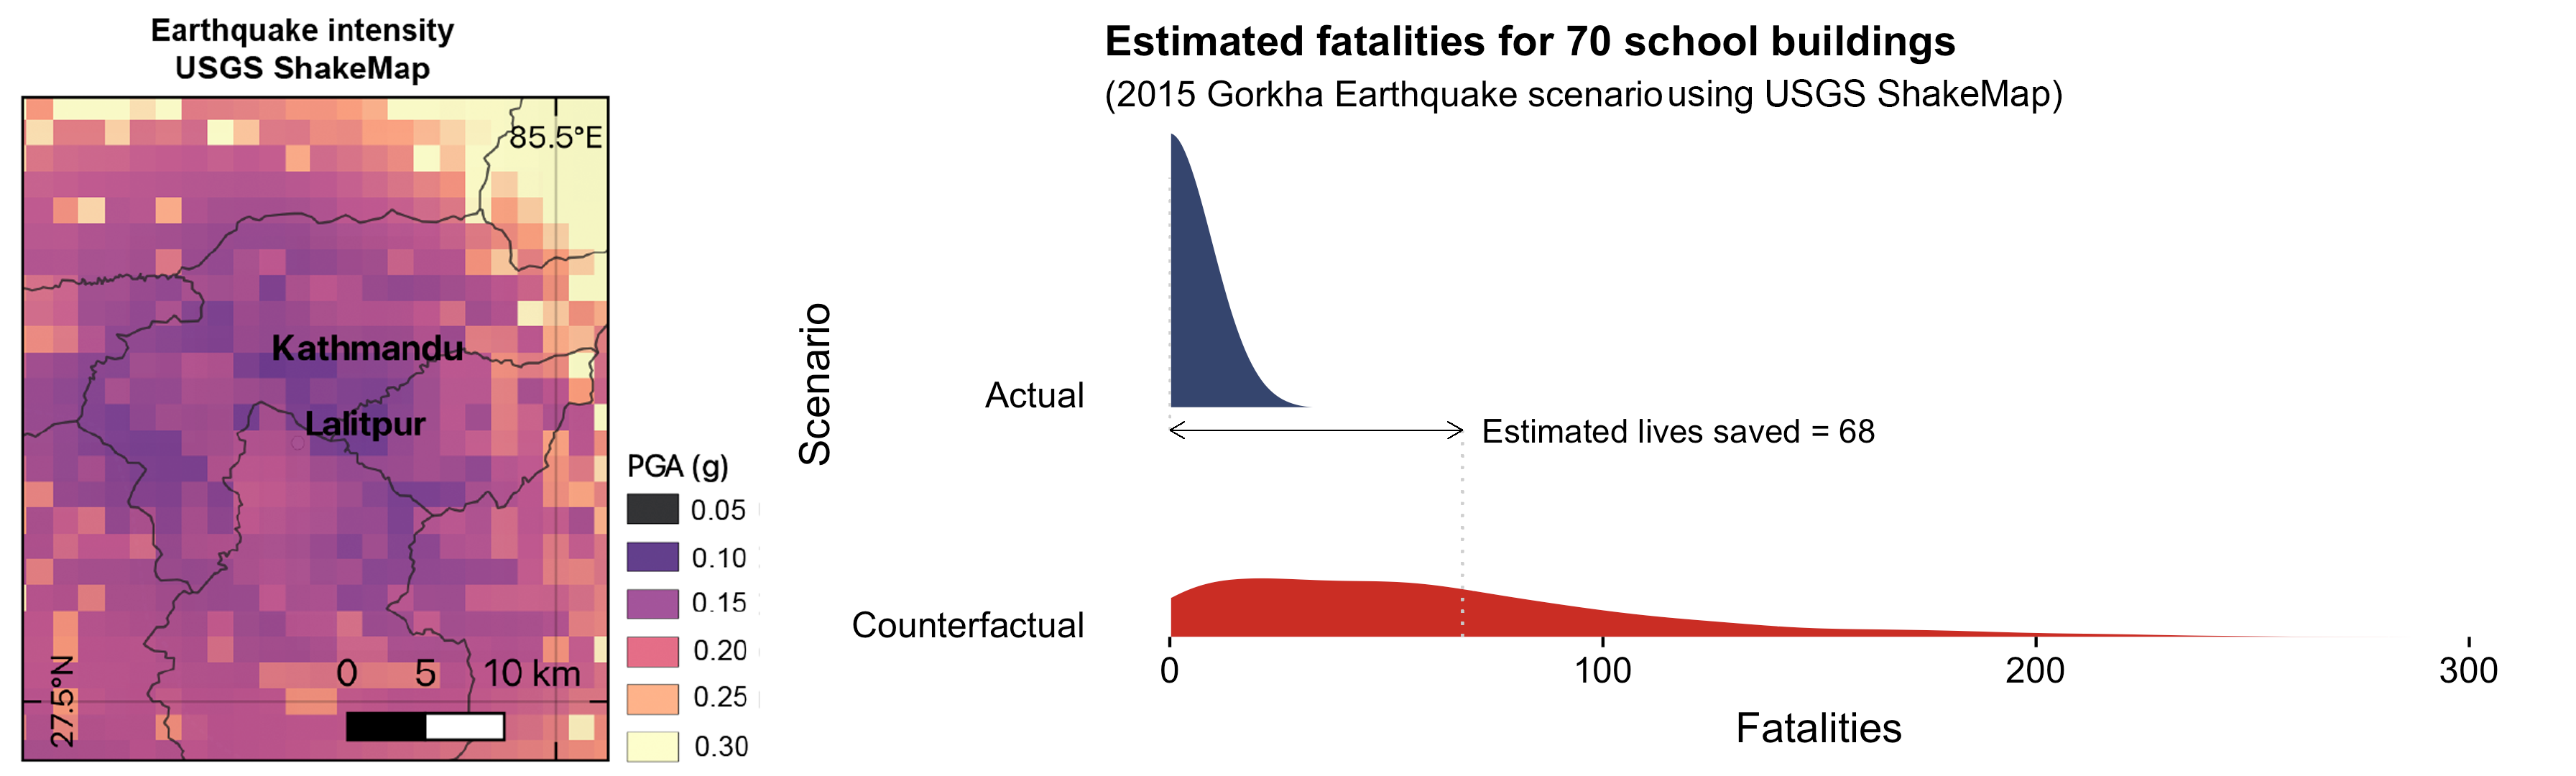
\includegraphics[width=\linewidth]{Figures/results_case-shakemap-compile.png}
		\caption{A re-analysis of the case study described in Section 5.1 is performed using the peak ground acceleration map for the 2015 $M_{w}$ 7.8 Gorkha earthquake obtained from \cite{shakemap2015nepal} (shown on the left). Using this hazard model, our analysis show an estimated of 68 lives saved in the 70 retrofitted schools.}
	\label{fig:supplementary_ShakeMap}
	\end{center}
    \end{figure}


\section{Relevant first-author publication for Chapter 4} \label{app-pls-2}

\noindent
Cited in Chapter 4 is a paper published as a Contributing Paper to the Global Assessment Report (GAR) on Disaster Risk Reduction 2022 by the United Nations Office for Disaster Risk Reduction (UNDRR)
\\ \\
\noindent
\textbf{Rabonza, M.L.}, Lallemant,  D.,  Lin,  Y. C., Tadepalli,  S., Wagenaar,  D., Nguyen,  M., Choong,  J., Liu,  C. J. N., Sarica,  G. M., Widawati,  B. A. M., Balbi,  M., Khan,  F., Loos,  S. \& Lim,  T. N. (2022). Shedding light on avoided disasters : measuring the invisible benefits of disaster risk management using probabilistic counterfactual analysis. \textit{A contributing paper to the United Nations Office for Disaster Risk Reduction (UNDRR) Global Assessment Report 2022}. https://www.undrr.org/publication/shedding-light-avoided-disasters-measuring-invisible-benefits-disaster-risk-reduction

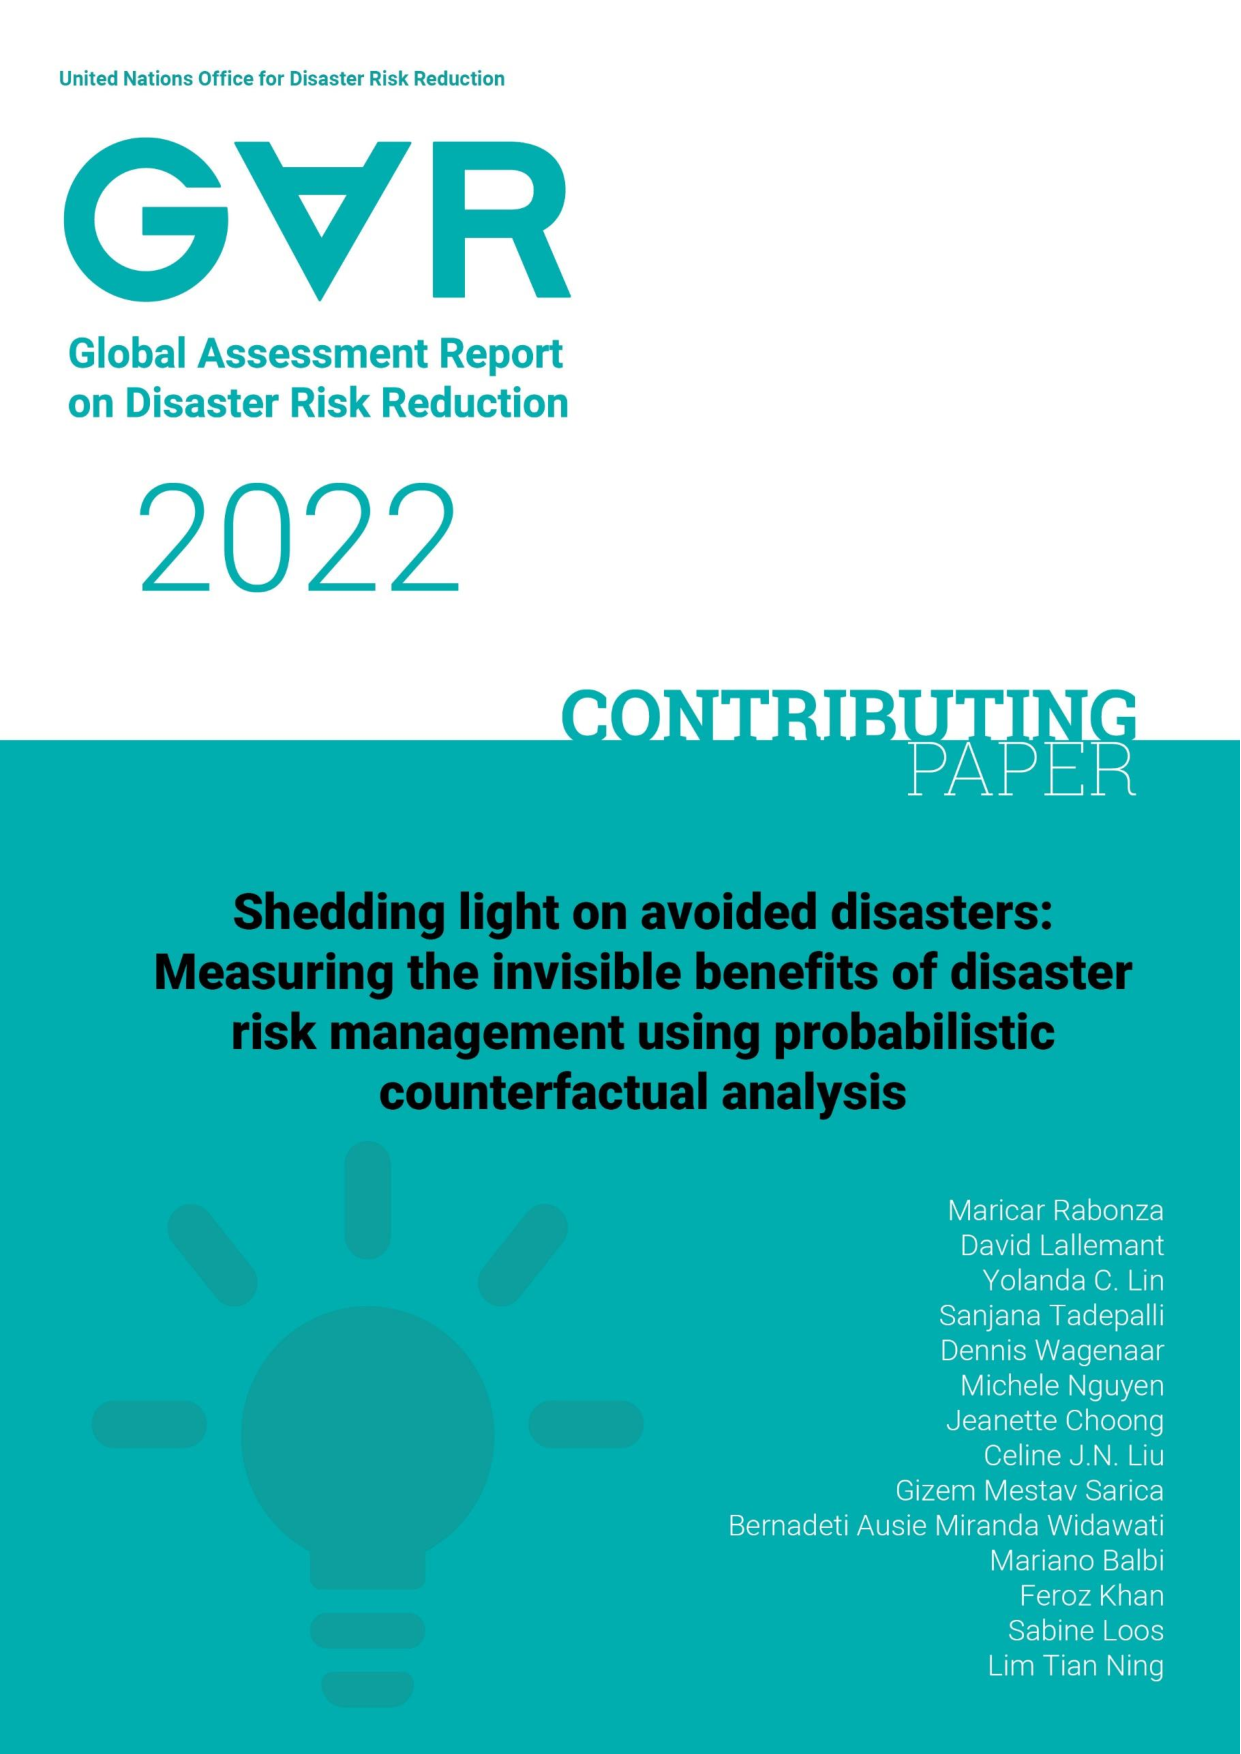
\includepdf[pages=-, scale=0.8, pagecommand=\thispagestyle{plain}]{GAR_published.pdf}